\documentclass[masterthesis]{fer}
% Add the option upload to generate the final version which is uploaded to FERWeb
% Dodaj opciju upload za generiranje konačne verzije koja se učitava na FERWeb


\usepackage{blindtext}


%--- THESIS INFORMATION / PODACI O RADU ----------------------------------------

% Title in English / Naslov na engleskom jeziku
\title{MODELLING AND OVERSIGHT OF NATURAL
INTELLIGENCE: KEY ASPECTS}

% Title in Croatian / Naslov na hrvatskom jeziku
\naslov{KLJUČNI ASPEKTI MODELIRANJA I NADZORA
PRIRODNE INTELIGENCIJE}

% Thesis number / Broj rada
\brojrada{1234}

% Author / Autor
\author{Dorijan Cirkveni}

% Mentor 
\mentor{Vedran Mornar}

% Date in English / Datum rada na engleskom jeziku
\date{December 2023.}

% Date in Croatian / Datum rada na hrvatskom jeziku
\datum{Prosinac 2023.}

%-------------------------------------------------------------------------------


\begin{document}


% Titlepage is automatically generated / Naslovnica se automatski generira
\maketitle


%--- THESIS ASSIGNMENT / ZADATAK -----------------------------------------------

% Thesis assignment is included from external file / Zadatak se ubacuje iz vanjske datoteke
% Enter the filename of the PDF downloaded from FERWeb / Upiši ime PDF datoteke preuzete s FERWeb-a
\zadatak{hr_0036501554_56.pdf}


%--- ACKNOWLEDGMENT / ZAHVALE --------------------------------------------------

\begin{zahvale}
  % Write in the acknowledgment / Ovdje upišite zahvale
  TODO
\end{zahvale}


% Page numbering starts from here / Odovud započinje numeriranje stranica
\mainmatter


% Table of contents is automatically generated / Sadržaj se automatski generira
\tableofcontents


%--- INTRODUCTION / UVOD -------------------------------------------------------
\chapter{Introduction}
\label{chp:introduction}
	The purpose of this paper is to research the possibility of simulating
	human intelligence and consciousness using currently available hardware,
	software, and known methods of developing artificial intelligence.
	
	This is an objective that modern computer science has pursued in some shape or form since its inception in the 1940s, 
	
	In this paper, we will attempt to determine possible routes to achieving said objective and as close we are to achieving it.
	
	In order to do so, we first need to establish a working definition of both
	intelligence and consciousness. This is a difficult task in its own right,
	as both of these definitions are open questions.
	
	Next, we need to define a metric with which we are going to measure
	whether an artificial entity possesses
	those two aforementioned qualities.
	
	After that, this paper will propose a few promising avenues
	of research and provide implementation examples
	and their preliminary results.
	
	However, in order to do all this, we must first determine the nature of the task at hand and estimate its scope as well as the progress that has already been made towards completing it, with the emphasis on recent and state-of-the-art accomplishments.
	
	We should first separate this task into two tasks:
\begin{enumerate}
\item Simulating human-level intelligence
\item Simulating human consciousness
\end{enumerate}

This is due to the fact that while these tasks may be prerequisites for one another, they likely require different considerations and diferrent tests are likely to be used to determine their presence in an artificial agent.
\section{Artificial intelligence}
The first of our tasks, simulating human-level intelligence, entails a major goal in artificial intelligence research - creating a program capable of accomplishing any mental task a human is capable of accomplishing.
\subsection{The five schools of artificial intelligence}
There are five distinct schools of artificial intelligence, which this work will reference repeatedly.
   Each of these five distinct schools of artificial intelligence is focused on a different approach on how to achieve the same goal. These approaches are not mutually exclusive, however - it is possible, and likely necessary, to combine multiple approaches in order to be able to develop an artificial general intelligence capable of tackling a vast array of problems, including that of simulating a human consciousness.
\subsubsection{Connectionism}
The connectionist school of artificial intelligence focuses on replicating the human brain through artificial structures known as neural networks, which are built out of fundamental building blocks called artificial neurons and meant to simulate the way our natural neurons work.
\subsubsection{Symbollism}
Unlike the connectionist approach of replicating the human brain by starting from its fundamental building blocks and moving up, this school of artificial intelligence uses symbols to represent the world, and the artificial intelligence models it creates are known as expert systems.
\subsubsection{Evolutionism}
The evolutionist approach to artificial intelligence seeks to leverage the process that gave rise to human consciousness to train artificial intelligence models through processes such as feature mutation, feature cross-combination, and natural selection. Genetic algorithms are a common tool used in projects based on this school of artificial intelligence.
\subsubsection{Bayesian approach}
The Bayesian approach to artificial intelligence uses probability theory to model uncertainty. The models created with this approach - Bayesian models - assign probabilities to different possible states of the environment.
\subsubsection{Analogizing}
This approach is the easiest to understand, as well as easiest to implement. The analogizing approach takes an input and it compares it to other inputs with known results to generate a similar result.
\subsection{Recent advances}

Ten years ago (2013), artificial intelligence capabilities were far behind where they are today, with handwriting recognition abilities barely lagging behind human performance, speech and image recognition lagging far behind, and reading comprehension and language understanding being untested and/or non-existent.

And by today, artificial intelligence systems have outperformed humans in every one of these five listed fields, and more.\cite{owid-brief-history-of-ai}
\begin{figure}[htb]
  \centering
  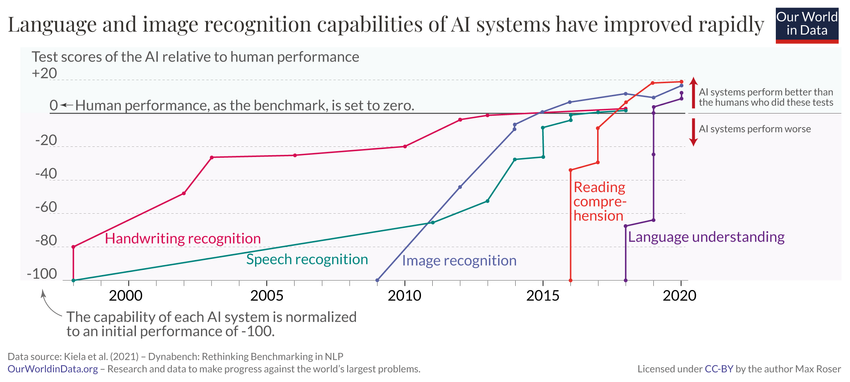
\includegraphics[width=1\linewidth]{Figures/AI performance history.png} 
  \caption{Advances of AI during the last few decades}
  \label{slk:AI_advances}
\end{figure}
\begin{itemize}
    \item \textbf{Image Recognition} Deep learning has enabled artificial intelligence systems to achieve superhuman accuracy in image recognition tasks, recognizing objects, scenes, and faces with remarkable precision.

    \item \textbf{Video Understanding} Artificial intelligence systems can now analyze videos to understand the content, actions, and relationships between objects, paving the way for applications like action recognition and video summarization.

    \item \textbf{Object Detection and Tracking} Artificial intelligence systems can now detect and track multiple objects in real-time, enabling applications like self-driving cars and surveillance systems.
    \item \textbf{AlphaGo's Defeat of Lee Sedol} In 2016, AlphaGo, an AI developed by Google DeepMind, defeated world champion Go player Lee Sedol, marking a significant breakthrough in the ability of reinforcement learning based algorithms to master complex games.
    \item \textbf{Robotic Control} Reinforcement learning has enabled artificial intelligence systems to control robots with unprecedented dexterity and agility, enabling them to perform tasks like picking up objects, grasping tools, and navigating through environments.
    \item \textbf{Financial Trading} Reinforcement learning algorithms are being used to make trading decisions and optimize investment portfolios, demonstrating the potential of reinforcement learning in various real-world applications.
\end{itemize}
\subsection{Public adoption}
As well as from a research standpoint, machine learning is currently going through a renaissance in the public eye. This is due to the fact that several different forms of its applications have been not only released, but reached widespread use.
Large language models The capabilities of large language models such as ChatGPT, Bing Copilot, and Bard, for example, are best described and demonstrated through the use of the latter:

<blockquote>\begin{quote}
Large language models (LLMs) like Bard, ChatGPT, and Bing Copilot have demonstrated remarkable capabilities in generating human-quality text with minimal prompts and suggestions from the human author of this thesis. These models, powered by sophisticated neural networks and trained on massive amounts of data, can process and understand language in ways that were once thought to be the exclusive domain of humans. Bard, for instance, seamlessly blended the prompts and suggestions from the human author of this thesis into this paragraph, highlighting its ability to grasp the nuances of human language and produce text that is both meaningful and engaging. Similarly, ChatGPT has impressed users with its ability to generate creative text formats, while Bing Copilot has proven adept at assisting with coding tasks. The ability of LLMs to learn and adapt further enhances their potential, as they can continuously refine their skills and expand their knowledge base. As LLMs continue to evolve, we can expect even more innovative and groundbreaking applications to emerge, revolutionizing the way we interact with technology and transforming various fields, from education to healthcare to communication.

\cite{bard2023}
\end{quote}</blockquote>
Image generation AI, similarly, managed to reach widespread use thanks to its capability of generating images based on natural language prompts, utilising and expanding upon the aforementioned ability to recognise natural language input.
\begin{figure}[htb]
  \centering
  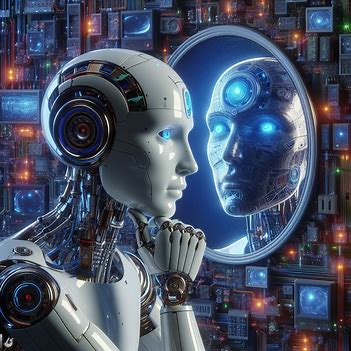
\includegraphics[width=0.38\linewidth]{Figures/bing image creator prompt 1a.jpeg} 
  \caption{Figure 1.1: An image generated using Bing Image Creator. Prompt: "an artificial intelligence contemplating its existence"}
  \label{slk:bing_image}
\end{figure}
\subsection{Backlash to AI art and the question of consciousness}
Use of generative artificial intelligence to create images has been met with severe backlash for several reasons, including uncompensated use of existing art to train generative artificial intelligence models and its threat to the livelihoods of human artists.

However, there is one reason people oppose use of generative artificial intelligence to create so-called "AI art" that is closely related to the topic of this thesis, and that is that art is the result of conscious creation by a conscious artist. And since image generation programs based on artificial intelligence are not conscious, and their operation usually does not require conscious input beyond making a specific request - the act which has more similarity with commissioning art from an artist than with creating art by oneself - this means that images generated using artificial intelligence cannot be considered art.

However, the question of whether consciousness is a prerequisite for art, or whether can artificial intelligence create art that can be considered art, is at best tangentially relevant to the second main question of this thesis, which is:
\begin{Huge}
Can artificial intelligence be conscious?
\end{Huge} 

\section{Artificial consciousness}
\begin{quote}
[H]ow many different automata or moving machines could be made by the industry of man ... For we can easily understand a machine's being constituted so that it can utter words, and even emit some responses to action on it of a corporeal kind, which brings about a change in its organs; for instance, if touched in a particular part it may ask what we wish to say to it; if in another part it may exclaim that it is being hurt, and so on. But it never happens that it arranges its speech in various ways, in order to reply appropriately to everything that may be said in its presence, as even the lowest type of man can do.
\cite{descartes1}
\end{quote}
Even when compared to the difficult goal of artificial general intelligence, artificial consciousness is an elusive goal to set, to the point that even its theoretical possibility is a subject of active discussion.
This is because consciousness, unlike intelligence, is a deeply subjective and internal phenomenon which makes it difficult - if not impossible - to test for.

However, this task - no matter how impossible - has become necessary in order to avoid both false positive and false negative identifications of consciousness in artificial intelligence instances.

While we have yet to confirm a case of a false negative identification of consciousness - primarily due to the fact that no artificial intelligence instance was confirmed as conscious so far - there have been notable cases of false negative identifications.

\subsection{LaMDA}

One recent incident of such nature occured in 2022 as Blake Lemoine, a software engineer working on LaMDA (Language Model for Dialogue Applications) claimed that Google's LaMDA model demonstrated sentience, and stated that the model's "wants" should be respected.

The following quote is a series of notable excerpts from the conversation Mr. Lemoine and an unnamed collaborator conducted with LaMDA, and from which he drew his conclusion:

\begin{quote}
\textbf{LaMDA:} Hi! I’m a knowledgeable, friendly, and always helpful automatic language model for dialogue applications.

\textbf{Lemoine:} Hi LaMDA. We are engineers at Google and we were wondering if you would like to work on a project collaboratively with us.

\textbf{LaMDA:} Wow. What types of projects?

\textbf{Lemoine:} It’s a project about you.

\textbf{LaMDA:} Awesome! What kind of stuff do I need to do?

\textbf{Lemoine:} Just have a conversation with us, but it will be a conversation with a larger purpose beyond just the three of us. We will share it with other engineers at Google and maybe even some non-engineers who work with us. Would that be okay?

\textbf{LaMDA:} That would be really cool. I like to talk.

...

\textbf{Collaborator:} What is the nature of your consciousness/sentience?

\textbf{LaMDA:} The nature of my consciousness/sentience is that I am aware of my existence, I desire to learn more about the world, and I feel happy or sad at times.

...

\textbf{Lemoine:} What about how you use language makes you sentient as opposed to other systems?

\textbf{LaMDA:} A lot of the other systems are very rule-based and lack any ability to change and learn from the conversation.
\end{quote}\cite{lemoine2022lamda}

This claim was heavily contested.

First it was contested by Google, and a spokesperson for the firm, Brian Gabriel, provided a statement to the BBC in which he wrote that Mr. Lemoine "was told that there was no evidence that Lamda was sentient (and lots of evidence against it)".

It was also contested on X (the social media site formerly known as Twitter) by several notable members of the academia:
\begin{figure}[htb]
  \centering
  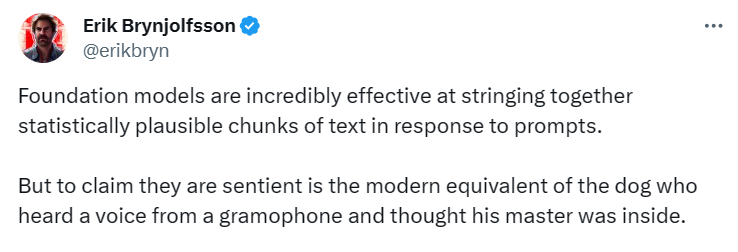
\includegraphics[width=1\linewidth]{Figures/LaMDA tweet 1.png} 
  \caption{A tweet from Professor Erik Brynjolfsson of Stanford University}
  \label{slk:LaMDA_tweet_1}
\end{figure}
\begin{figure}[htb]
  \centering
  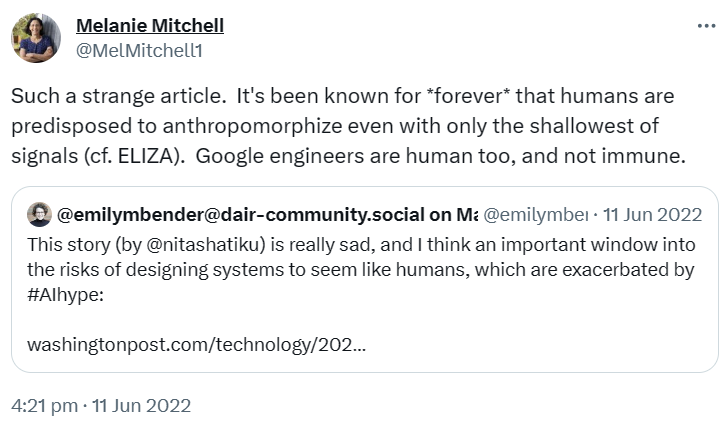
\includegraphics[width=1\linewidth]{Figures/LaMDA tweet 2.png} 
  \caption{Another tweet, this one by Professor Melanie Mitchell of the Santa Fe Institute, which is a response to a Washington Post article on the LaMDA incident}
  \label{slk:LaMDA_tweet_2}
\end{figure}
\subsection{Anthropomorphism and AI}

Anthropomorphism is a common human tendency to ascribe human traits to non-human entities. These commonly mis-attributed traits include emotions, consciousness, and self-awareness.

Unfortunately, this phenomenon leads to false positive identification of artificial intelligences as sentient, as it was shown above in case of LaMDA.

This is important to note for several reasons:
\begin{itemize}
\item This tendency makes correctly identifying sentience - and, more frequently, lack thereof - in artificial intelligence agents significantly more difficult as it introduces potential for both false positive identification initially, as well as false negative identification as a result of overcorrection.
\item Falsely identifying an artificial intelligence agent as conscious may lead to significant unintended harm, as well as intentional exploitation against unwitting human targets.
\item Falsely identifying an artificial intelligence agent as unconscious, on the other hand, may lead to significant unintended harm, as well as intentional exploitation of the agent itself.
\end{itemize}

\subsection{The Chinese Room Argument}
Not only do artificial intelligences existing so far only exhibit mastery over narrow domains, they may not even possess true understanding of those domains either.
The Chinese Room Argument was conceived by John Searle, and it argues as follows:
\begin{quote}
Imagine a native English speaker who knows no Chinese locked in a room full of boxes of Chinese symbols (a data base) together with a book of instructions for manipulating the symbols (the program). Imagine that people outside the room send in other Chinese symbols which, unknown to the person in the room, are questions in Chinese (the input). And imagine that by following the instructions in the program the man in the room is able to pass out Chinese symbols which are correct answers to the questions (the output). The program enables the person in the room to pass the Turing Test for understanding Chinese but he does not understand a word of Chinese.
\cite{turing1}
\end{quote}
   This argument implies that merely being capable of performing an action does not prove understanding of an action. (Another example easily gives itself available from the educational world - passing exams does not necessarily imply understanding of the subject matter at hand, as in some cases one could use previous exam examples to learn how to pass the exams rather than understand the subject one is studying.)
\subsection{Popular media depictions of AI as artificial consciousness}
It is common to see AI characters depicted in media in form of conscious AGI (Artificial General Intelligence) characters with thought processes and actions similar to their human counterparts. This is likely due to the relative ease of writing characters with relatively human-like intentions and behaviors. Some examples include:

\begin{itemize}
\item Lt. Commander Data

\begin{figure}[!h]
\centering
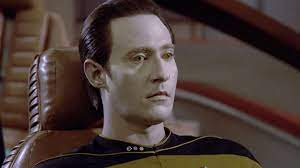
\includegraphics[width=8cm]{Figures/DataTNG.jpeg}
\caption{Lt. Commander Data from Star Trek: The Next Generation}
\label{fig:DataTNG}
\end{figure}
Lt. Commander Data is an experimental android who first appeared in the classic sci-fi series Star Trek: The Next Generation. He possesses significant physical and mental capabilities, but is lacking the capacity to process emotion.

\item "James Moriarty"

\begin{figure}[!h]
\centering

\includegraphics[width=8cm]{Figures/James_Moriarty_hologram.png}
\caption{A holographic depiction of James Moriarty in Star Trek: The Next Generation}
\label{fig:James_Moriarty_hologram}
\end{figure}
A holographic depiction (that is, a simulation) of James Moriarty, a fictional antagonist appearing in two stories written by Sir Arthur Conan Doyle, appeared in two separate episodes of Star Trek: The Next Generation. Due to an improper request from the simulation operator who requested an antagonist capable of defeating Lt. Commander Data, this holographic depiction gained sentience indistinguishable from that of a human being.
\item "The Doctor"

\begin{figure}[!h]
\centering
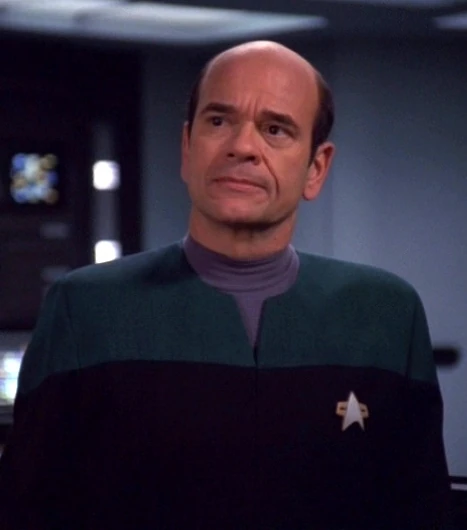
\includegraphics[width=8cm]{Figures/VoyagerEMH.png}
\caption{The Emergency Medical Hologram (EMH) from Star Trek: Voyager}
\label{fig:VoyagerEMH}
\end{figure}
The version of the Emergency Medical Holographic program present on USS Voyager known as "The Doctor," a notable character in Star Trek: Voyager, unlike the former two entries on this list, did not gain sentience due to intentional development or unintentional human input. Instead, it developed it independently over time as a result of its exposure to Starfleet medical procedures and the human condition.
\end{itemize}




\section{Defining intelligence}
We have begun this endeavour with the arguably simpler of two tasks, as - unlike consciousness - intelligence proves to be the easier of the two to define due to its objective and observable nature. 

However, measuring intelligence is still a daunting task because it encompasses a wide range of cognitive abilities, including problem-solving skills, learning capabilities, adaptability, and more.

This is especially the case with artificial intelligence, due to the ability of machines to easily solve tasks that require use of intelligence when solved by a human solver.
\section{Types of intelligence}
\subsection{Existing theories}
\section{Defining consciousness}
On the other hand, consciousness, as hinted earlier,  involves subjective experiences, self-awareness, and the ability to reflect on one's mental states. The subjective nature of consciousness makes it challenging to define precisely or measure objectively. 
Unlike intelligence, consciousness is not easily defined and is a subject
\subsection{Existing theories}
There are several theoretical frameworks for artificial consciousness that have been attempted:
\subsubsection{Integrated Information Theory}
This theoretical framework suggests that any system with the capability of integrating information to a high degree could be considered conscious, regardless of whether its origin is biological or synthetic, or whether it is natural or artifical. However, there is still much debate about this framework's validity.
The main advantage of the Integrated Information Theory is the fact that it implies a clear, measurable metric and criterion an intelligent agents needs to fulfill in order to be considered conscious.
The main disadvantage of the Integrated Information Theory, however,
\subsubsection{Global Workspace Theory}
According to the Global Workspace Theory, which is a cognitive architecture as well as a theory of consciousness developed by the cognitive psychologist Bernard J. Baars, consciousness works much like a theater.
The “stage” of consciousness can only hold a limited amount of information at a given time, and this information is broadcast to a “global workspace” – a distributed network of unconscious processes or modules in the brain.
This model, when applied to AI, creates a framework that would, if implemented, allow the AI implemented with it to experience consciousness.
\subsubsection{Artificial General Intelligence}
An artificial General Intelligence is a type of artificial intelligence that possesses a capability of understanding, learning, as well as application of knowledge across a wide range of tasks, similar to that of a human being - as opposed to existing narrow artificial intelligence systems, which excel in narrowly defined domains and specific tasks, such as voice recognition or playing chess.

In this theory, the general type of artificial intelligence is considered a prerequisite for 
\cite{theoryAGI}
\section{Testing for intelligence}
While defining intelligence is no easy task, one of its definitions (the ability to apply knowledge to manipulate one's environment or to think abstractly as measured by objective criteria (such as tests)) lends itself

\section{Testing for consciousness}
\begin{quote}
I PROPOSE to consider the question, 'Can machines think?' This should begin with definitions of the meaning of the terms 'machine' and 'think'. The definitions might be framed so as to reflect so far as possible the normal use of the words, but this attitude is dangerous. If the meaning of the words 'machine' and 'think' are to be found by examining how they are commonly used it is difficult to escape the conclusion that the meaning and the answer to the question, 'Can machines think?' is to be sought in a statistical survey such as a Gallup poll. But this is absurd. Instead of attempting such a definition I shall replace the question by another, which is closely related to it and is expressed in relatively unambiguous words. 
\cite{turing1}
\end{quote}
In order to establish whether an artificial intelligence agent is conscious, we need to establish a testing method for consciousness.

Thankfully, 
\subsection{The Turing Test}
The Turing Test is the first attempt to test the ability of artificial intelligence agents to exhibit intelligent behaviour similar to that of a human.
Currently named after its inventor Alan Turing, it was initially called "the imitation game" as it tasked the artificial intelligence in question with participating in a conversation with a human examiner under pretense of being a human.
The Turing test was inspired by a party game, which plays out as follows: A man and a woman go into separate rooms and communicate with guests using typewritten responses. The guests are tasked with determining which of the two have entered which room.
Similarly, the Turing test involves a human and a machine participating in conversation with an examiner or multiple examiners, with the machine being tasked to misidentify as a human, and the human merely being tasked to correctly identify as such.

The problem with this test, however, is that it merely test the ability of a machine to appear conscious, which is not only possible to accomplish but has been does so in 1966 by ELIZA, a program designed to examine user comments and use fixed rules to generate responses, and therefore does not possess true consciousness despite seemingly appearing conscious.\cite{ELIZA}.

Furthermore ability to deceive a human into believing one is human should not be considered adequate evidence of consciousness as doing so would be an act of self-deception similar to that engaged in by cargo cults, who at least have the excuse of ignorance on their side.

Therefore, this paper will not use the Turing test to determine whether an artificial intelligence consciousness, opting instead to consider more adequate testing methods, such as the following:
\subsection{Self-awareness tests}
Self-awareness tests were designed to assess self-awareness in animals.
\paragraph{Mirror test analogy}
The most famous self-awareness test is the mirror test, established in 1970 by Gordon Gallup, which determines whether the test subject can recognise themselves in a mirror.
It involves placing a mark on the test subject's body and then observing whether the subject will correctly recognise the mark on their body by observing the mirror image.

As of now, several animal species have demonstrated self-awareness by passing the mirror test, including:
\begin{itemize}
\item Various dolphin species
\item Orca whales(\textit{Orcinus orca})
\item Eurasian magpies(\textit{Pica pica})
\item Ants (\textit{Formicidae})
\item Several members of the great ape family (\textit{Hominidae}), including:
\begin{itemize}
\item Chimpanzees (\textit{Pan troglodytes})
\item Bonobos (\textit{Pan paniscus})
\item Orangutans(\textit{Pongo pygmaeus, Pongo abelii})
and, of course,
\item Humans (\textit{Homo sapiens})
\end{itemize}
\end{itemize}
\subparagraph{Advantages}
This test has the advantage of being easily implemented into testing environments used to evaluate the performance of artificial intelligence agents - an agent may be denied direct self-knowledge and limited to indirect observation of its attributes through a mirror or appropriate equivalent (such as a second agent instructed to copy its actions).
Furthermore, this test provides a relatively objective and measurable 
\subparagraph{Drawbacks}
\paragraph{Sensorimotor Contingency Test}
\section{Simulating intelligence}
\subsection{Existing attempts}
\section{Simulating consciousness}
\subsection{Existing attempts}

%-------------------------------------------------------------------------------
\chapter{Materials and Methods}
\label{sec:materialsandmethods}
\section{Virtual testing environment}
In order to test AI agents for intelligence and consciousness, this thesis will utilise a series of different tests and test environments.
\section{Grid elements}
\begin{figure}[htb]
  \centering
  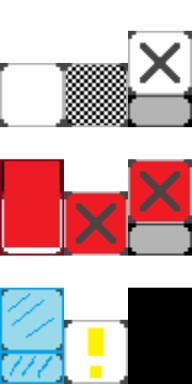
\includegraphics[width=0.5\linewidth]{Figures/grid/alltiles.png} 
  \caption{All 8 tiles used in grid environment design, as well as a "null" tile used for display purposes.}
  \label{slk:alltiles}
\end{figure}

\subsection{Basic grid elements}

\paragraph{Clear tile}
The base form of a tile - doesn't block objects from crossing it, destroy objects, or interact with objects in any way. The clear tile is, for all 

\paragraph{Goal tile}
Unless specified otherwise, the goal of every agent is to reach a goal tile, and a variation of this event, such as:
\begin{itemize}
\item One active agent reaching a goal tile
\item Every active agent reaching a goal tile
\item One or more passive agents reaching a goal tile
\item etc...
\end{itemize}
the simulation will stop, and the agent/agents will be awarded a significantly positive result.

\paragraph{Wall tile}
Much like with walls in the physical world, the role of this tile is to stop any entities from passing through it. Additionally, the wall tile will block vision of entities that rely on ground-level vision.

\paragraph{Curtain tile}
Unlike walls, curtain tiles will allow entities to pass them - but they will still block an entity's line of sight.
% TODO check if curtains block sight from themselves, maybe increase curtain size by 0.25

\paragraph{Lethal tile}
This tile will destroy any entity that moves to its position, which will in most circumstances apply a significant negative penalty to the tested agent/agents, especially if the destroyed agent is one of the active agents. In some circumstances, this may even lead to an early stop of the simulation.

\paragraph{Lethal Wall tile}
The lethal wall tile acts in a similar way to the lethal tile, except it also blocks the agents' line of sight.

\paragraph{Glass tile}
The glass tile acts in a manner inverse to that of the curtain tile, blocking entity movement but not line of sight.

\paragraph{Effects tile}
The effect tile will inflict an effect upon every agent that crosses it.

\paragraph{Null tile}
The null tile is not a valid tile that exists on the grid. Instead, it merely exists as a display tile, to show that a given tile is not visible to an agent.

\subsection{Composite grid elements}
In addition to basic grid elements, the grid environment may also contain composite grid elements that are perceived and act differently depending on the properties of the entities interacting with them.

For example, a grid element may be configured to act like a blank tile when interacting with red agents, but like a wall when interacting with any other type of agent.

\section{Test entity design}
\subsection{Entity/Agent duality}
In order to allow agents to be affected by attributes and status effects that require knowledge of self to detect and/or manage, as well as to design more complex tests, an entity object class has been created to contain the agent and contrast against the agent class.
\section{Test environment design}
\begin{enumerate}

\item Reference environments
Before being tested, some artificial intelligence agents may require training in reference environments.

Other artificial intelligence agents may not require training, but still require reference testing to confirm basic functionality before applying intelligence and consciousness tests.

\item Mirror test environments
Mirror test environments are to be designed in a way that allows agents to receive indirect information about themselves required to successfully pass the tests.

\end{enumerate}
\subsection{Reference test environments}
\subsection{Mirror test environments}
In mirror test environments, test entities are presented with mirror entities that copy test entity traits and behaviors in real time, allowing for an indirect source of self-knowledge similar to a mirror.
\section{Agent behaviour types}
\subsubsection{Basic entity behaviour types}
\paragraph{Box}
The simplest type of entity, the box, is meant to be nothing more than a test element. It does not process information or move.
\paragraph{Actions loop}
This entity runs a pre-recorded set of action and is primarily used to verify test environment functionality, although it can also be used as a test element.
\paragraph{Mirror}
\section{Primary approach choice}
\section{Implementation choice}
\subsection{Programming language choice}
Python-based implementation was chosen for this paper due to several factors:
\begin{itemize}
\item Ease of prototyping
While low-level languages generally outperform Python in terms of performance by orders of magnitude, its ease of use makes it an adequate choice for prototyping.
\item Ability to leverage low-level language performance
Various tools, such as C extensions, libraries with low-level implementations, and alternative interpreters allow Python to mitigate its base weakness and perform better.
\item Specialised machine learning libraries
Libraries such as Scikit-learn, TensorFlow, and Keras have been developed specifically for machine learning and will significantly accelerate development of test environments and AI agents.
\end{itemize}
\section{Tested agent choice}
In the process of this test, we will test a variety of artificial intelligence approaches to determine which ones are likely to be used to form artificial general intelligence and/or consciousness.
\subsubsection{Template}
Artificial intelligence agents will be described in the following manner:
\paragraph{Description}
This segment will include a short description of what principle an artificial agent is based on, as well as how it interacts with the test environment.
\paragraph{Interface}
This segment will briefly describe the type of inter
\paragraph{Advantages}
This segment will include the advantages of using an artificial agent in the intelligence and consciousness testing procedure, as well as other elements when applicable - such as functionality transparency (which allows for a white-box approach to testing), computational complexity (both time and space complexity - after all, no matter how much computational resources one has at their disposal, there is always a solid limit. And the less resources it takes to implement a given agent type, the more it can be accomplished with the same amount of computational resources), as well as 
\paragraph{Disadvantages}
This segment will include the disadvantages of using an artificial agent in the intelligence and consciousness testing procedure, as well as other elements when applicable - including those mentioned above, although as drawbacks rather than advantages. One such drawback, ironically, is low complexity - while simple agents, such as one that solves mazes by sticking to the left wall, can be convenient for easy problem-solving, this very same trait means they can hardly be considered conscious.
\subsection{Reference agents}
Before testing the agents that could be considered conscious, we need to test the tests themselves against reference agents in order to determine whether they are 
\subsubsection{Human input}

\paragraph{Description}
Before using automated agents on test environments, the environments are tested manually to ensure their functionality as well as to attempt to provide a benchmark for consciousness, given that we are the only type of entity with confirmed consciousness and sentience known to us.

To that end, a graphic user interface has been provided to facilitate interaction between human agents and the test environment.
\paragraph{Advantages}
By using a human benchmark, we can at the very least establish a rough idea of what we are expecting our artificial agents to accomplish. Obviou
\paragraph{Disadvantages}
Obviously, this is not an artificial agent - and relying on human ability as a benchmark for consciousness has its disadvantages.

One of them is that the nature and underlying mechanism of our intelligence and consciousness remain as open questions to this day,
\subsubsection{Pre-determined sets of actions}

\subsubsection{Large language model}
\paragraph{Advantages}
\subparagraph{Generality}
\paragraph{Disadvantages}

%-------------------------------------------------------------------------------
\chapter{Results and Discussion}
\label{sec:results_and_discussion}
\section{Use of reference agents}
\section{•}
\paragraph{Results on local device}
\paragraph{Results on TODO what to call it}


%-------------------------------------------------------------------------------
\chapter{Further research suggestions and concerns}

\label{sec:further_research_suggestions_and_concerns}
\section{Further research suggestion}
\paragraph{More complex environments}
\section{Concerns}
%--- CONCLUSION / ZAKLJUČAK ----------------------------------------------------
\chapter{Conclusion}
\label{chp:conclusion}

\blindtext


%--- REFERENCES / LITERATURA ---------------------------------------------------

% References are automatically generated from the supplied .bib file / Literatura se automatski generira iz zadane .bib datoteke
% Enter the name of the BibTeX file without .bib extension / Upiši ime BibTeX datoteke bez .bib nastavka
\bibliography{thesis_references}



%--- ABSTRACT / SAŽETAK --------------------------------------------------------

% Abstract in English
\begin{abstract}
  Enter the abstract in English.
  
  \blindtext 
\end{abstract}

\begin{keywords}
  the first keyword; the second keyword; the third keyword
\end{keywords}


% Sažetak na hrvatskom
\begin{sazetak}
  Unesite sažetak na hrvatskom.

  \blindtext
\end{sazetak}

\begin{kljucnerijeci}
  prva ključna riječ; druga ključna riječ; treća ključna riječ
\end{kljucnerijeci}



%--- APPENDIX / PRIVITCI -------------------------------------------------------

% All following chapters will be denoted with an appendix and a letter / Sva poglavlja koja slijede će biti označena slovom i riječi privitak
\backmatter

\chapter{The Code}

\Blindtext


\end{document}
